\section{Workflow Abstraction}

\label{sec:abstraction}
The main purpose of the work done so far for workflow abstraction is related with the creation of a trie structure which captures the sequences of execution of a workflow and keeps track of their statistics. A trie is an ordered tree that stores a dynamic set of keys where they usually are strings. For our purposes we have used it for storing the workflow execution in an ordered way by including at different levels of the tree the different inputs, processes and outputs (resources) which are run. Therefore all the descendants of a node have a common prefix of the resource associated with that node. This is very useful for detecting common parts of different workflows beause we can easily keep track of the number of times that an specific sequence of resources has been executed. \\

We want to highlight that the goal of making an abstraction of a workflow is to make them more reusable as a whole or some parts of it. Then, we define abstraction as the sequence of resources which are executed together and by a minimum number of times. This definition leads also to the concept of pattern or macro identification which applied to workflows leads to finding common sub-workflows. \\ 

The presented work is a bottom-up approach in order to study the actual provenance of workflow results (which represents the dataflow of an executed workflow) from a set of available workflows at WINGS~\url{http://wings.isi.edu/} and Taverna~\url{http://www.taverna.org.uk/} created for this purpose. The description of the provenance of workflow results and wfprov ontology can be found at~\cite{D4.2v1} and \url{http://purl.org/wf4ever/wfprov#} respectively, and an example of a RO containing the provenance of workflow results for the Protein Discovery Workflow is available \url{http://sandbox.wf4ever-project.org/portal/ro?0&ro=http://sandbox.wf4ever-project.org/rosrs5/ROs/wf74/} which is part of the RO testbed \url{http://www.wf4ever-project.org/wiki/display/docs/RO+testbed}. \\


This study uses the provenance of the workflow results of different workflows as inputs for creating the trie structure introduced above. Every time a resource is executed its associated node in the trie structure is updated by increasing the number of times that it has been used and afterwards an analysis of the trie can be done to obtain the most common set of resources or macros. \\
 

Though this is still a preliminary work, once a set of macros have been identfied it would be possible to categorize them (manually or automatically p.e. by using workflow tags) and afterwards create the associated taxonomy by using the trie membership relations.

The use of the provenance of the workflow results seems to be more appealing that using the workflow templates, which are the static description of workflow (see Section \ref{sec:model} ), mainly due to it represents the workflows which are actually running and being used, and also allows to undo control structures as p.e. "if".

The code developed for the creation and maintance of the trie structure and for accesing to the provenance of the workflow results repository is availabe at \url{https://github.com/wf4ever/wf-abstraction} and provides the following funcionality:

\begin{itemize}
\item It stores the provenance of the workflow results in an ordered way and the appearance frequency of their resources
\item It calculates relative frecuencies at different levels of the trie
\item It provides different modes to traverse the structure (pre-ordered/level-orderred)
\item It provides an output XML structure with relative frecuencies per level and per process (an output example is available at \url{https://github.com/wf4ever/wf-abstraction/blob/master/outputExample.xml})
\end{itemize}

The Figure~\ref{fig:workflowAbstraction} shows the overall discovery process introduced in this section. The inputs have been obtained by using workflows from WINGS and Taverna and transforming them into wfdesc and wfprov vocabularies to get the provenance of workflow results. That provenance has been stored in a trie structure which captures the order of the executed resources and stores the frecuencies of appearance. Then, that information can be used to obtain the most frequent set of ordered executed resources which we have called macros and are identified in the figure of the bottom by black squares. Afterwards these detected macros, which represent some common workflow structures, could be hand-annotated in order to tag them or could be annotated automatically for example by assigning to them the same tags as the workflows that they belong to. Finally a taxonomy which includes all the identified macros by membership (bigger macros contain the smaller ones) will be created fo indexing purposes.

\begin{figure}
\begin{center}
\label{fig:workflowAbstraction}
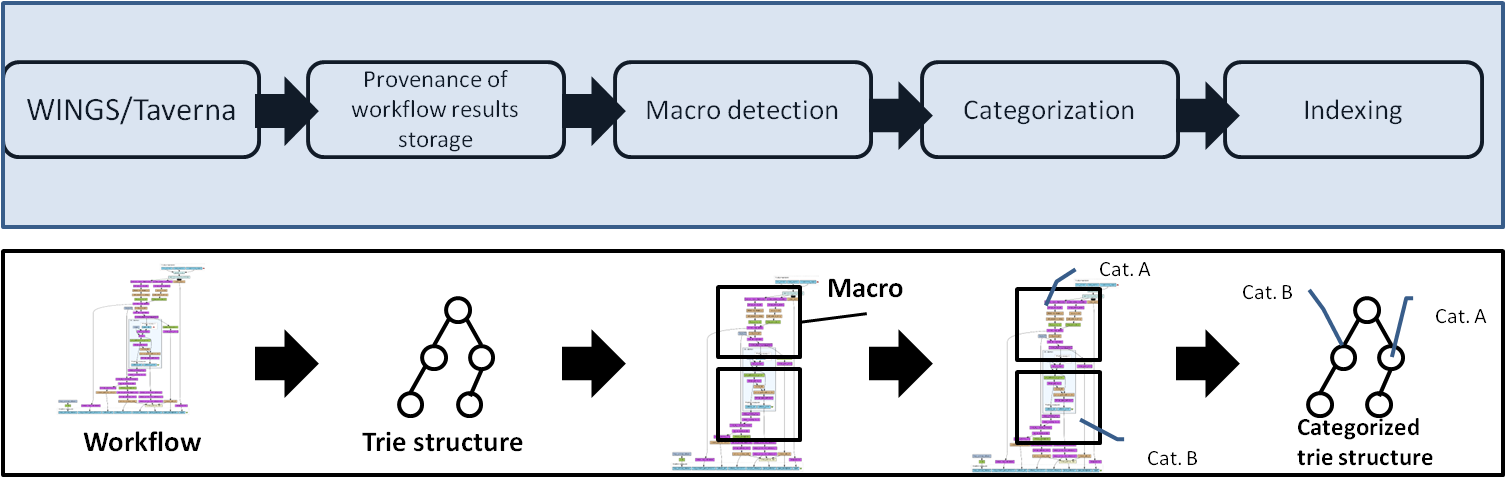
\includegraphics[scale=0.5]{./Figures/workflowAbstraction}
\caption{Workflow Abstraction Discovery Process}
\end{center}
\end{figure}